	\chapter{Datenanalyse}\label{sec:Datenanalyse}
	In dieser Seminararbeit wird eine Analyse von Wohnungspreisen in 20 deutschen Städten durchgeführt. Der Datensatz wurde durch Webscraping von der Website Immonet.de gewonnen und enthält Informationen wie Größe, Preis, Anzahl der Zimmer und Lage der Wohnungen. Um die Datenqualität zu verbessern, wurden bestimmte Filtereinstellungen verwendet und einige Daten manuell korrigiert.
	
	Im ersten Schritt der Datenanalyse werden potentielle Ausreißer identifiziert und untersucht. Dazu werden statistische Methoden und grafische Darstellungen verwendet, um ungewöhnliche oder unplausible Daten zu erkennen. Im zweiten Schritt werden die erhaltenen Ergebnisse interpretiert und mögliche Gründe für die Ausreißer untersucht.
	
	Zuvor erfolgt eine Beschreibung des Datensatzes.
	
	
	\section{Beschreibung des Datensatzes}
	Die Beschreibung des Datensatzes ist der Tabelle \ref{tbl: vor der Analyse} zu entnehmen. Die Tabelle zeigt den Datensatz vor der Analyse. Dazu wurden die folgenden Spaltenüberschriften gewählt. 
	\begin{description}
		\item[Variable] Die Bezeichnung der ausgelesenen Variablen. Die Angaben in Klammern sind die 
		Bezeichnungen der 'Spaltennamen' in dem Datensatz.
		
		\item[Str] Die Struktur der Variablen. Dabei steht:
		\begin{description}
			\item[fac] für Faktoren bzw. kategoriale Variablen.
			
			\item[chr] Für Character - 'Text' Variablen
			
			\item[num] Numerische Daten.
			
			\item[date] Datumsformat
			
			
		\end{description}
		\item[Anzahl/Ausprägungen] Bei numerischen Werten sind es  die Anzahl der Datensätze. Bei kategorialen Daten sind es die Anzahl der Kategorien.
		
		\item[Median] Der Median der numerischen Daten.
		\item[Range] Bei Kategorialen Variablen werden die verschiedenen Kategorien mit der Anzahl der verfügbaren
		Daten für diese entsprechende Kategorie angegeben. Voraussetzung ist, dass eine kategoriale Variable weniger als
		10 Ausprägungen hat. Bei numerischen Daten wird der kleinste und größte Wer ausgegeben
		\item[NA] NA steht für not available. Diese Daten wurden in den Inseraten nicht angegeben.
		\item[Anmerkung] Persönlische Anmerkung
		
	\end{description}

\begin{landscape}
	\begin{tabular}{|l||c|c|c|l|l|} \hline
		Variable         & str  & Anzahl/Ausprägungen & Median	    	& Range                          & NA \\ \hline \hline
		Preis       	 & num  & 5912                & 401.450      	& 75.000 - 3.100.000             & - \\  \hline
		ID               & chr  & 5912                &			    	& -                              & -\\ \hline
		Zimmer           & num  & 5912                & 2.5  	    	& 1 - 42                         & -\\ \hline
		Fläche           & num  & 5912                &	72.5$m^2$    	& 16.9 - 1456                    & -\\ \hline
		Ort      		 & fac	& 88                  &				    & Adlershof ... Zehlendorf       & -  \\ \hline
		Zustand    		 & fac	& 11                  &				    & Altbau... Vollsaniert          & -  \\ \hline
		Art              & fac  & 9                   &    				& Apartment: 103                 & - \\ 
						&      &                     &	    			& Dachgeschosswohnung: 443       & \\
						&      &                     &    				& Erdgeschosswohnung: 586        & \\
						&      &                     &    				& Etagenwohnung: 3628            & \\
						&      &                     &	    			& Loft-Studio-Atelier: 94        & \\
						&      &                     &	    			& Maisonette: 159                & \\
						&      &                     &	    			& Penthouse: 135                 & \\
						&      &                     &	    			& Souterrainwohnung: 25          & \\
						&      &                     &	    			& Dachgeschosswohnung: 443       & \\
						&      &                     &	    			& Wohnung: 736                   & \\ \hline
		Fotos 		    & num  & 5913                &	12	    		& 0 - 42                         & - \\ \hline
		Baujahr         & Date & 150                 & 1960   			& 1838 - 2025                    & 694 \\ \hline
		Denkmalschutz   & bool & 2                   &	    			& True: 213                      &  \\ 
						&      &                     &    				& False: 5699                    &  \\ \hline
		Energieklasse   & fac  & 9                   &    				& Klasse A+ - Klasse H           & 3291   \\ \hline
		Energieverbrauch& num  &                     &	104.2  kWh/(m²*a)& 1 - 190949                    & 1672   \\ \hline
Energieverbrauchsausweis & fac  & 3                   &	                 & Energiebedarfsausweis: 1815   &     \\ 
						&      &                     &	                 & Energieverbrauchsausweis: 2478  &  1427   \\ 
						&      &                     &	                 & nicht nötig:192               &     \\ \hline
			Heizungsart & fac  & 3                   &	                 & Etagenheizung: 458            &      \\ 
						&      &                     &	                 & Zentralheizung: 2468          &      \\ \hline
		Befeuerungsart  & fac  & 30                  &	                 & Erdwärme,Solar... Gas         & 1002 \\ \hline
		Ausstattung     & num  & 5912                &	  25             & 1-376         		         &  52  \\ \hline
		Objekt          & num  & 5912                &	  129            & 2-492         		         &   262  \\ \hline
		Lage            & num  & 5912                &	  104            & 1-529         		         &   396  \\ \hline
		Sonstiges       & num  & 5912                &	  62             & 0-501         		         &   371  \\ \hline
		Dokumente       & num  & 5912                &	  1             & 1-5           		         & 4236  -  \\ \hline
	\end{tabular}
\caption{Datensatz vor der Analyse}
\label{tbl: vor der Analyse}
\end{landscape}
\section{Ausreißeranalyse}\label{sec:Ausreißeranalyse}

Die Ausreißeranalyse dient dazu, mögliche Abweichungen oder Fehler im Datensatz aufzudecken. Durch die Identifizierung von Ausreißern kann sichergestellt werden, dass die Ergebnisse der Analyse valide sind und auf einer stabilen Datenbasis beruhen. Es ermöglicht, die Datenqualität zu verbessern, indem diese Ausreißer entfernt oder korrigiert werden. Ziel der Ausreißeranalyse ist es also, die Daten auf Plausibilität zu überprüfen und dadurch die Zuverlässigkeit und Validität der Ergebnisse zu erhöhen.

\subsection{Kategoriale Daten}

\subsubsection{Stadt}
Es wurden Daten von 20 Städten ausgelesen. Dabei ist festzustellen, dass im Osten Deutschlands mehr Wohnimmobilien zur Verfügung stehen als in Garmisch-Partenkirchen, wo lediglich 8 Immobilien vorhanden sind. Trotzdem werden diese Daten beibehalten, da in Zukunft regelmäßige Aktualisierungen stattfinden und eine Analyse der Performance im Laufe der Zeit erfolgen soll. Daher ist es wichtig, die Stadt Garmisch-Partenkirchen in dem Datensatz zu berücksichtigen.

\begin{verbatim}
Garmisch-Partenkirchen                Potsdam                   Kiel 
                     8                     26                     53 
                 Mainz              Wiesbaden            Saarbrücken 
                    80                    106                    107 
              Schwerin              Stuttgart                 Erfurt 
                   161                    186                    208 
                Bremen             Düsseldorf               Hannover 
                   212                    235                    242 
             Frankfurt                 Berlin                München 
                   318                    421                    493 
              Nürnberg                Hamburg                Leipzig 
                   574                    727                    750 
             Magdeburg                Dresden 
                   753                    861 
\end{verbatim}

\subsubsection{Art}

Bei der Überprüfung auf Plausibilität der Daten fiel auf, dass einige Wohnungen lediglich als 'Wohnung' bezeichnet wurden. Hier besteht die Möglichkeit, dass es sich trotz der Kategorie 'Wohnung', um eine andere Art der Wohnung handelt. Um diese Daten zu spezifizieren, müssten Textpassagen der Inserate analysiert werden.

\begin{verbatim}
Loft-Studio-Atelier   Souterrainwohnung           Penthouse          Maisonette 
                 25                  30                  90                 184 
          Apartment  Erdgeschosswohnung Dachgeschosswohnung             Wohnung 
                531                 617                 621                1600 
      Etagenwohnung 
               2823 
\end{verbatim}


\subsubsection{Zustand der Immobilie}
Das primäre Ziel soll eine Vorhersage der Warm- und Kaltmiete auf Basis individuelle Eingaben erfolgen. Bei der Auswahl des Zustands der Immobilie ist es schwer vorstellbar, dass ein Individuum eine 'Entkernte Immobilie' sucht. Diese Daten wurden entfernt
\begin{verbatim}
                            Entkernt                          Projektiert 
                                   1                                    8 
Teil- oder vollrenovierungsbedürftig                               Altbau 
                                  12                                  263 
                              Neubau             Teil- oder vollrenoviert 
                                 338                                  643 
                           Neuwertig               Teil- oder vollsaniert 
                                 684                                  953 
                           Erstbezug                         keine Angabe 
                                1024                                 2595
\end{verbatim}

\subsubsection{Heizungsart, Energieklasse \& Energieverbrauchsausweis }
Bei den Daten zur Heizungsart, der Energieklasse oder dem Energieverbrauchsausweis sind keine Auffälligkeiten festzustellen

\begin{verbatim}
tbl %>% 
   select(energieklasse) %>%
   table() %>%
   sort(decreasing = F) 

Klasse H     Klasse G    Klasse A+     Klasse F     Klasse A     Klasse E 
      23           52          119          216          266          349 
Klasse C     Klasse D     Klasse B keine Angabe 
     506          636          759         3595 

tbl %>% 
   select(heizungsart) %>%
   table() %>%
   sort(decreasing = F) 

Ofenheizung  Etagenheizung   keine Angabe Zentralheizung 
         10            430           2570           3511 

tbl %>% 
   select(energieverbrauchsausweis) %>%
   table() %>%
   sort(decreasing = F) 

             nicht nötig             keine Angabe    Energiebedarfsausweis 
                     498                     1952                     1990 
Energieverbrauchsausweis 
                    2081 
\end{verbatim}


\subsection{Nummerische Daten}
Bei den nummerischen Daten wird zunächste für die Daten 'Warmmiete', 'Kaltmiete', 'Energieverbrauch' und 'Fläche' eine Normalverteilung unterstellt. Diese Unterstellung wird nicht durch weitere Hypothesentests untersucht. Das Ziel soll lediglich sein - die Daten einzeln betrachtet - dass einige Daten an den Rändern ausgeschlossen werden, wie beispielsweise die Warmmiete von 4.400.000 EUR aus der Abbildung \ref{Error: allgemeine Fehler}. Die Daten werden logarithmiert und dann skaliert, sodass der Mittelwert 0 und die Standardabweichung 1 beträgt. Im Anschluss an die Einzelbrachtung erfolgt noch eine Untersuchung der mahalanobis Distanz. Über die Distanzberechnung mehrdimensionaler Datensätze ist es möglich außergewöhnliche Daten zu identifizieren und zu entfernen. 

\subsubsection{Warmmiete}
Die kleinste Warmmiete beträgt 200 EUR. Die teuerste Warmmiete aller Daten beträgt 4.400.000 EUR. Es gibt 36 Datenpunkte die außerhalb des dreifachen der Standardabweichung liegen. Die graphische Darstellung im Vergleich mit der Normalverteilung ist in Abbildung \label{Ausreißer_vgl_warmmiete} zu sehen. Die Daten werden erst entfernt, wenn alle Daten untersucht worden sind.

\begin{figure}[h!]
	\centering
	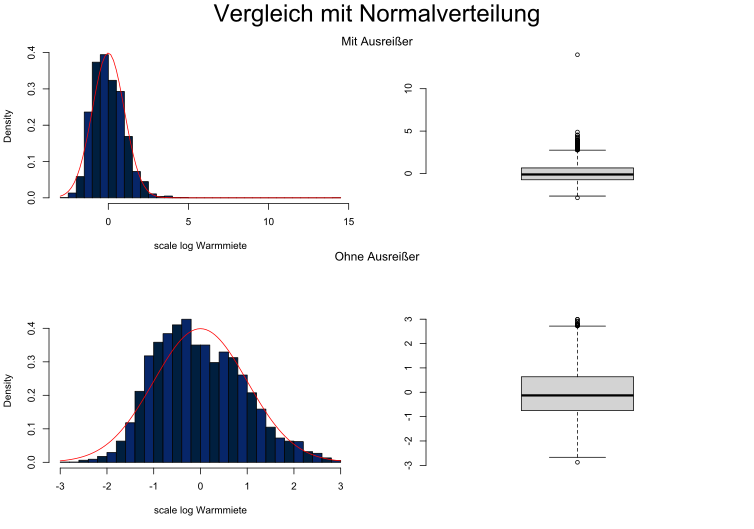
\includegraphics[width=1\linewidth]{img/Ausreißer_warmmiete.pdf}
	\caption{}
	\label{fig: Ausreißer_vgl_warmmiete}
\end{figure}


\subsubsection{Kaltmiete}
Für die Kaltmiete belief sich vor der Analyse auf einem Bereich von $[ 72 EUR ,  17.000 EUR]$. Ohne Ausreißer liegen die Kaltmieten im Intervall $[150 EUR, 5.820 EUR]$
\begin{figure}[h!]
	\centering
	\includegraphics[width=1\linewidth]{img/Ausreißer_kaltmiete.pdf}
	\caption{}
	\label{fig: Ausreißer_kaltmiete}
\end{figure}

\subsubsection{Energieverbrauch}

Für den Energieverbrauch stehen ca. 60 \% Daten zur Verfügung. In 40 \% der Fälle wurde keine Angabe zum Energieverbrauch gemacht. Für die restlichen 3.924 \% Daten ergibt sich das folgende Schaubild.

\begin{figure}[!h!]
	\centering
	\includegraphics[width=1\linewidth]{img/ausreißer_energieverbrauch.pdf}
	\caption{}
	\label{fig: Ausreißer_kaltmiete}
\end{figure}

51 Daten wurden als Ausreißer identifiziert.

\subsubsection{Fläche}
Die Spannweite der Fläche aller Daten beträgt 700 $m^2$. Die Daten liegen zwischen 7 und 700 $m^2$ . Für die Fläche wurden 73 Ausreißer identifiziert, sodass die sich die Spannweite auf 231 $m^2$ reduziert und die Daten nun im Intervall $[18.6 m^2 , 250 m^2 ]$ liegen.

\begin{figure}[h!!]
	\centering
	\includegraphics[width=1\linewidth]{img/ausreißer_energieverbrauch.pdf}
	\caption{}
	\label{fig: Ausreißer_flaeche}
\end{figure}

\subsubsection{Zimmer}


\begin{verbatim}
	> table(tbl$zimmer)
	
  1  1.5    2  2.5    3  3.5    4  4.5    5  5.5    6  6.5    7  7.5    8    9   10 
708   97 2458  201 2075  114  630   39  140   10   26    1   13    2    2    2    3 
\end{verbatim}
\begin{figure}[h!!]
	\centering
	\includegraphics[width=.6\linewidth]{img/ausreißer_zimmer.pdf}
	\caption{}
	\label{fig: ausreißer_zimmer}
\end{figure}
\subsection{Mahalanobis Distanz}
Die Mahalanobis Distanz berechnet die Distanz im mehrdimensionalen Vektorraum. Für die euklidische Ebene - also im zweidimensionalen Raum - lässt sich die Mahalanobis Distanz interpretieren, als der Abstand zweier Punkte. Wird dieses Vorgehen auf alle Daten angewandt ...


\section{Korrelationsanalyse}